% =============================================================================
% Final Review Presentation (Beamer Widescreen 16:9)
% Team Number: 15 | School of Computing, Amrita Vishwa Vidyapeetham
% Project: Robust 2D Plasma Equilibrium Reconstruction Under Sensor Failures
% Candidates: Kalidasan B (AM.SC.U4AIE24025) & Nishanth D (AM.SC.U4AIE24061)
% Supervisor: Dr. Simi S
% =============================================================================

\documentclass[aspectratio=169, 10pt]{beamer}

% ---------------- 1. Theme, Margins & Typography ----------------
\usetheme{Madrid}
\usefonttheme{professionalfonts}

% Clean 16:9 Margins (Maximizes horizontal width, controls vertical bounds)
\setbeamersize{text margin left=18pt, text margin right=18pt}

% Remove bulky top navigation header bar (Reclaims ~1.8cm vertical height)
\setbeamertemplate{headline}{}

% Remove default navigation symbols
\setbeamertemplate{navigation symbols}{}

% Slim, Elegant Custom Footline (Preserves slide height)
\setbeamertemplate{footline}{
  \leavevmode%
  \hbox{%
  \begin{beamercolorbox}[wd=.34\paperwidth,ht=2.2ex,dp=0.8ex,left]{author in head/foot}%
    \usebeamerfont{author in head/foot}\hspace*{2ex}Team 15: Kalidasan B \& Nishanth D
  \end{beamercolorbox}%
  \begin{beamercolorbox}[wd=.38\paperwidth,ht=2.2ex,dp=0.8ex,center]{title in head/foot}%
    \usebeamerfont{title in head/foot}Robust 2D Tokamak Equilibrium Reconstruction
  \end{beamercolorbox}%
  \begin{beamercolorbox}[wd=.28\paperwidth,ht=2.2ex,dp=0.8ex,right]{date in head/foot}%
    \usebeamerfont{date in head/foot}\insertframenumber{} / \inserttotalframenumber\hspace*{2ex}
  \end{beamercolorbox}}%
  \vskip0pt%
}

% ---------------- 2. Color Palette ----------------
\definecolor{NavyBlue}{RGB}{15, 44, 89}        % Primary Header & Accents
\definecolor{TealAccent}{RGB}{0, 141, 218}     % Secondary Accent
\definecolor{CharcoalText}{RGB}{30, 41, 59}    % Body Text
\definecolor{LightSlate}{RGB}{245, 247, 250}   % Background
\definecolor{DarkRed}{RGB}{180, 40, 40}        % Highlighting & Alerts
\definecolor{ForestGreen}{RGB}{34, 139, 34}    % Success & Best Results

\setbeamercolor{palette primary}{bg=NavyBlue, fg=white}
\setbeamercolor{palette secondary}{bg=TealAccent, fg=white}
\setbeamercolor{palette tertiary}{bg=NavyBlue, fg=white}
\setbeamercolor{structure}{fg=NavyBlue}
\setbeamercolor{titlelike}{bg=NavyBlue, fg=white}
\setbeamercolor{item}{fg=NavyBlue}

% Typography & Spacing
\setlength{\itemsep}{4pt}
\linespread{0.98}

% ---------------- 3. Packages ----------------
\usepackage[utf8]{inputenc}
\usepackage[T1]{fontenc}
\usepackage{lmodern}
\usepackage{amsmath,amssymb}
\usepackage{graphicx}
\usepackage{booktabs}
\usepackage{array}
\usepackage{multirow}
\usepackage{tikz}
\usetikzlibrary{arrows.meta, positioning, shapes.geometric, fit, backgrounds}
\usepackage{hyperref}

\hypersetup{
  colorlinks=true,
  linkcolor=NavyBlue,
  urlcolor=TealAccent,
  pdftitle={Team 15 - Robust 2D Tokamak Equilibrium Reconstruction},
  pdfauthor={Kalidasan B and Nishanth D}
}

% Table column width helpers (Guaranteed to fit 16:9 textwidth ~14.5cm)
\newcolumntype{P}[1]{>{\raggedright\arraybackslash}p{#1}}
\newcolumntype{C}[1]{>{\centering\arraybackslash}p{#1}}

% ---------------- Title Metadata ----------------
\title[Robust 2D Tokamak Equilibrium Reconstruction]{Robust 2D Tokamak Equilibrium Reconstruction\\from Sparse Wall Diagnostics Under Sensor Failure}
\subtitle{Evaluating Spatial and Temporal Deep Learning Baselines on TokaMark}
\author[Team 15]{Kalidasan B \inst{1} \and Nishanth D \inst{1}}
\institute[Amrita Vishwa Vidyapeetham]{
  \inst{1} School of Computing, Amrita Vishwa Vidyapeetham\\
  \vspace{3pt}
  \textbf{Supervisor:} Dr. Simi S \quad $\vert$ \quad \textbf{Team Number:} 15
}
\date{Academic Year 2026 -- Semester 5}

% =============================================================================
\begin{document}

% -----------------------------------------------------------------------------
% SLIDE 1: Title Slide
% -----------------------------------------------------------------------------
\begin{frame}[plain]
  \titlepage
\end{frame}

% -----------------------------------------------------------------------------
% SLIDE 2: Problem Statement: The Physical Challenge
% -----------------------------------------------------------------------------
\begin{frame}{1. Problem Statement: The Physical Confinement Challenge}
  \begin{columns}[T]
    \begin{column}{0.48\textwidth}
      \textbf{\color{NavyBlue} Magnetic Plasma Confinement}
      \begin{itemize}
        \item In a fusion tokamak, a \textbf{100-million-degree plasma} is confined inside a vacuum vessel using powerful magnetic fields.
        \item Physical probes cannot enter the plasma core without being vaporized.
        \item The entire internal magnetic state --- the \textbf{2D poloidal flux map $\boldsymbol{\psi(R, Z)}$} --- must be inferred purely from magnetic sensors mounted on the chamber walls.
      \end{itemize}
    \end{column}

    \begin{column}{0.48\textwidth}
      \textbf{\color{NavyBlue} Why Equilibrium Reconstruction Matters}
      \begin{itemize}
        \item $\psi(R, Z)$ determines the exact position, shape, and boundary of the plasma cross-section.
        \item Real-time boundary tracking is vital to prevent hot plasma from touching the reactor walls.
        \item Wall contact causes rapid heat loss, vessel wall melting, and destructive \textbf{plasma disruptions}.
      \end{itemize}
    \end{column}
  \end{columns}
\end{frame}

% -----------------------------------------------------------------------------
% SLIDE 3: Motivation & Limitations of Existing Solvers
% -----------------------------------------------------------------------------
\begin{frame}{2. Motivation \& Limitations of Existing Solvers}
  \begin{columns}[T]
    \begin{column}{0.48\textwidth}
      \textbf{\color{NavyBlue} Physics-Based Solvers (EFIT)}
      \begin{itemize}
        \item Standard tool across fusion reactors (MAST, JET, DIII-D).
        \item Solves the non-linear Grad-Shafranov differential equation iteratively.
        \item Accurate, but requires $\mathbf{50\text{--}500\text{ ms}}$ per slice --- far too slow for microsecond real-time control.
      \end{itemize}
    \end{column}

    \begin{column}{0.48\textwidth}
      \textbf{\color{NavyBlue} Deep Learning Surrogates}
      \begin{itemize}
        \item Neural networks learn direct mapping from wall sensors to 2D $\psi(R, Z)$.
        \item Executes in $<\!\mathbf{1\text{ ms}}$, enabling real-time feedback control.
        \item \textbf{The Catch:} Prior benchmarks evaluate models \textbf{only under idealized, 100\% clean sensor data}.
      \end{itemize}
    \end{column}
  \end{columns}
\end{frame}

% -----------------------------------------------------------------------------
% SLIDE 4: The Operational Reality: Harsh Reactor Environments
% -----------------------------------------------------------------------------
\begin{frame}{2b. Operational Reality: Harsh Reactor Environments}
  \begin{columns}[T]
    \begin{column}{0.48\textwidth}
      \textbf{\color{NavyBlue} Why Real Sensors Degrade and Fail}
      \begin{itemize}
        \item Intense $14\text{ MeV}$ neutron flux damages internal coil wiring.
        \item Severe thermal cycling causes integrator calibration drift.
        \item Reactor mechanical vibrations cause loose physical connections.
        \item Transient electrical arcs saturate Analog-to-Digital Converter (ADC) rails.
      \end{itemize}
    \end{column}

    \begin{column}{0.48\textwidth}
      \textbf{\color{NavyBlue} The Core Research Questions}
      \begin{itemize}
        \item What happens to deep learning 2D plasma reconstruction when wall sensors fail during operation?
        \item Does the reconstructed magnetic boundary warp, triggering false emergency shutdowns?
        \item Can online signal imputation prevent boundary collapse in real time?
      \end{itemize}
    \end{column}
  \end{columns}
\end{frame}

% -----------------------------------------------------------------------------
% SLIDE 5: Project Objectives: Modeling & Benchmark
% -----------------------------------------------------------------------------
\begin{frame}{3a. Project Objectives: Core Modeling \& Benchmark}
  \begin{columns}[T]
    \begin{column}{0.48\textwidth}
      \textbf{\color{NavyBlue} Objective 1: Sub-Millisecond 2D Reconstruction}
      \begin{itemize}
        \item Train deep neural surrogates to reconstruct the full 2D poloidal flux field $\psi(R,Z)$ on a $65 \times 65$ spatial grid ($4,225$ physical points).
        \item Achieve inference latency $<1\text{ ms}$ for real-time plasma shape control.
        \item Map from 8 heterogeneous wall sensor diagnostics.
      \end{itemize}
    \end{column}

    \begin{column}{0.48\textwidth}
      \textbf{\color{NavyBlue} Objective 2: Spatial vs. Temporal Benchmark}
      \begin{itemize}
        \item Conduct a rigorous head-to-head comparison between:
          \begin{enumerate}
            \item \textbf{CNN+MLP:} Spatial feedforward architecture.
            \item \textbf{CNN+LSTM:} Temporal recurrent architecture.
          \end{enumerate}
        \item Evaluate on the official UKAEA TokaMark benchmark protocol to identify the optimal baseline.
      \end{itemize}
    \end{column}
  \end{columns}
\end{frame}

% -----------------------------------------------------------------------------
% SLIDE 6: Project Objectives: Robustness & Mitigation
% -----------------------------------------------------------------------------
\begin{frame}{3b. Project Objectives: Robustness \& Live Mitigation}
  \begin{columns}[T]
    \begin{column}{0.48\textwidth}
      \textbf{\color{NavyBlue} Objective 3: First 2D Sensor Failure Benchmark}
      \begin{itemize}
        \item Stress-test trained models under 6 physical sensor failure modes (Gupta 2026 scenarios).
        \item Evaluate Gaussian noise, thermal calibration drift, cable dropouts, stuck ADC rails, and category outages.
        \item Test strictly on unseen experimental plasma discharges.
      \end{itemize}
    \end{column}

    \begin{column}{0.48\textwidth}
      \textbf{\color{NavyBlue} Objective 4: Online Fault Mitigation}
      \begin{itemize}
        \item Empirically evaluate real-time imputation strategies:
          \begin{itemize}
            \item \textbf{Zero-fill:} Default missing-value baseline.
            \item \textbf{Mean-fill:} Historical training average.
            \item \textbf{Forward-fill:} Physics-informed last-valid hold.
          \end{itemize}
        \item Discover which method prevents magnetic boundary breakdown during live plasma operations.
      \end{itemize}
    \end{column}
  \end{columns}
\end{frame}

% -----------------------------------------------------------------------------
% SLIDE 7: Literature Review - Part A
% -----------------------------------------------------------------------------
\begin{frame}{4a. Literature Review: Classical Solvers vs. Early Neural Nets}
  \vspace{-2pt}
  \begin{table}[h]
    \centering
    \small
    \renewcommand{\arraystretch}{1.2}
    \begin{tabular}{P{3.0cm} P{5.1cm} P{5.1cm}}
      \toprule
      \textbf{Study / Year} & \textbf{Approach \& Capabilities} & \textbf{Limitations \& Gaps} \\
      \midrule
      \textbf{Lao et al.} (1985, 1990) & EFIT physics inversion solving non-linear Grad-Shafranov equation. Gold standard. & Highly compute-intensive ($50\text{--}500\text{ ms}$); too slow for microsecond shape control. \\
      \addlinespace[6pt]
      \textbf{Ferreira et al.} (2020) & Classical MLPs for rapid equilibrium reconstruction on TCABR tokamak. & Small private dataset; assumes 100\% clean, noise-free sensor signals. \\
      \addlinespace[6pt]
      \textbf{Degrave et al.} (DeepMind, 2022) & Deep Reinforcement Learning for magnetic control on TCV (*Nature*). & Assumes perfect, uninterrupted state feedback; no sensor degradation analysis. \\
      \bottomrule
    \end{tabular}
  \end{table}
\end{frame}

% -----------------------------------------------------------------------------
% SLIDE 8: Literature Review - Part B
% -----------------------------------------------------------------------------
\begin{frame}{4b. Literature Review: Modern Benchmarks \& Robustness Studies}
  \vspace{-2pt}
  \begin{table}[h]
    \centering
    \small
    \renewcommand{\arraystretch}{1.2}
    \begin{tabular}{P{3.0cm} P{5.1cm} P{5.1cm}}
      \toprule
      \textbf{Study / Year} & \textbf{Approach \& Capabilities} & \textbf{Limitations \& Gaps} \\
      \midrule
      \textbf{Rousseau et al.} (UKAEA / IBM, 2026) & TokaMark foundation benchmark on 11,000+ MAST discharges (565 GB). & \textbf{Evaluated strictly on clean data}; zero sensor-failure testing. \\
      \addlinespace[6pt]
      \textbf{Gupta} (arXiv 2607.11915, Jul 2026) & Formulated 6 realistic sensor failure scenarios on TokaMark. & \textbf{Only tested Task 4-4 (1D scalar current forecasting)}; no 2D spatial field analysis. \\
      \addlinespace[6pt]
      \textbf{Yang et al.} (FusionMAE, 2025) & Masked Autoencoder for missing diagnostic channel imputation on HL-3. & Signal-level imputation only; not evaluated on 2D magnetic flux field quality. \\
      \bottomrule
    \end{tabular}
  \end{table}
\end{frame}

% -----------------------------------------------------------------------------
% SLIDE 9: Literature Review - The Identified Research Gap
% -----------------------------------------------------------------------------
\begin{frame}{4c. The Core Research Gap Addressed}
  \begin{columns}[T]
    \begin{column}{0.48\textwidth}
      \textbf{\color{NavyBlue} Research Gap 1: 2D Spatial Equilibrium}
      \begin{itemize}
        \item 1D scalar forecasting (Task 4-4) is fundamentally different from \textbf{2D spatial field reconstruction (Task 1-3)}.
        \item In a 2D field, sensor failure does not merely change a number --- it can distort the magnetic boundary, shift the axis, and hallucinate false X-points.
        \item No prior study has evaluated sensor degradation on 2D tokamak equilibrium fields.
      \end{itemize}
    \end{column}

    \begin{column}{0.48\textwidth}
      \textbf{\color{NavyBlue} Research Gap 2: Spatial vs. Temporal Models}
      \begin{itemize}
        \item Equilibrium reconstruction is physically instantaneous (Markovian).
        \item However, vacuum vessel walls carry delayed eddy currents.
        \item Prior literature has not resolved whether a memoryless model (\textbf{CNN+MLP}) or a recurrent model (\textbf{CNN+LSTM}) is more resilient when sensors drop out.
      \end{itemize}
    \end{column}
  \end{columns}
\end{frame}

% -----------------------------------------------------------------------------
% SLIDE 10: Scientific Novelty
% -----------------------------------------------------------------------------
\begin{frame}{5a. Scientific Novelty of This Project}
  \begin{columns}[T]
    \begin{column}{0.48\textwidth}
      \textbf{\color{NavyBlue} 1. First 2D Spatial Robustness Benchmark}
      \begin{itemize}
        \item Extends sensor failure stress-testing from simple 1D alarms to continuous 2D physical vector fields ($65 \times 65 = 4,225$ spatial points).
        \item Evaluates physical boundary distortion under 6 operational failure modes.
      \end{itemize}
      \vspace{4pt}
      \textbf{\color{NavyBlue} 2. Controlled Architecture Benchmark}
      \begin{itemize}
        \item Direct, apples-to-apples comparison between spatial feedforward (\textbf{CNN+MLP}) and temporal recurrent (\textbf{CNN+LSTM}) architectures on identical splits.
      \end{itemize}
    \end{column}

    \begin{column}{0.48\textwidth}
      \textbf{\color{NavyBlue} 3. Diagnostic Criticality Hierarchy}
      \begin{itemize}
        \item Systematically identifies which diagnostic channels are safety-critical versus which have built-in spatial redundancy.
      \end{itemize}
      \vspace{4pt}
      \textbf{\color{NavyBlue} 4. Real-Time Mitigation Discovery}
      \begin{itemize}
        \item Identifies that physics-informed \textbf{forward-fill imputation} preserves boundary topology during unexpected sensor dropouts.
      \end{itemize}
    \end{column}
  \end{columns}
\end{frame}

% -----------------------------------------------------------------------------
% SLIDE 11: Specific Engineering Contributions
% -----------------------------------------------------------------------------
\begin{frame}{5b. Technical Contributions by Our Team}
  \begin{columns}[T]
    \begin{column}{0.48\textwidth}
      \textbf{\color{NavyBlue} 1. Automated Kaggle Benchmark Pipeline}
      \begin{itemize}
        \item Engineered a robust training and evaluation pipeline on Kaggle Dual Tesla T4 GPUs processing 40 GB of official TokaMark data.
        \item Solved Kaggle multiprocessing shared-memory deadlocks by enforcing single-process data loading (`DL_WORKERS = 0`).
      \end{itemize}
      \vspace{4pt}
      \textbf{\color{NavyBlue} 2. Solved Subset Memorization}
      \begin{itemize}
        \item Identified severe overfitting on subset training; tuned Adam weight decay to $10^{-3}$, improving test MAE by \textbf{23\%}.
      \end{itemize}
    \end{column}

    \begin{column}{0.48\textwidth}
      \textbf{\color{NavyBlue} 3. Dual Architecture Implementation}
      \begin{itemize}
        \item Implemented and verified both \textbf{CNN+MLP} and \textbf{CNN+LSTM} models under the official TokaMark evaluation protocol.
      \end{itemize}
      \vspace{4pt}
      \textbf{\color{NavyBlue} 4. Complete Robustness Suite}
      \begin{itemize}
        \item Built a modular corruption engine (`robustness.py`) supporting Gaussian noise, drift, dropouts, and stuck ADC rails with zero-fill, mean-fill, and forward-fill recovery.
      \end{itemize}
    \end{column}
  \end{columns}
\end{frame}

% -----------------------------------------------------------------------------
% SLIDE 12: Dataset Details - The FAIR-MAST Archive
% -----------------------------------------------------------------------------
\begin{frame}{6a. Dataset Details: The FAIR-MAST Archive}
  \begin{columns}[T]
    \begin{column}{0.48\textwidth}
      \textbf{\color{NavyBlue} Benchmark Source \& Physical Origin}
      \begin{itemize}
        \item \textbf{Source:} TokaMark v1.0 (FAIR-MAST Database, UK Atomic Energy Authority / IBM Research / STFC).
        \item \textbf{Total Archive:} 11,188 experimental plasma discharges (565.3 GB) in cloud-native Zarr format.
        \item \textbf{Physical Origin:} Real magnetic and diagnostic measurements from the Mega Ampere Spherical Tokamak (MAST) in Culham, UK.
      \end{itemize}
    \end{column}

    \begin{column}{0.48\textwidth}
      \textbf{\color{NavyBlue} Our Budgeted Benchmark Subset (40 GB)}
      \begin{itemize}
        \item \textbf{Total Extracted:} 740 experimental shots ($\approx 40\text{ GB}$):
          \begin{itemize}
            \item \textbf{Training Split:} 606 shots (32.04 GB)
            \item \textbf{Validation Split:} 74 shots (3.98 GB)
            \item \textbf{Testing Split:} 60 shots (3.96 GB)
          \end{itemize}
        \item \textbf{Strict Shot-Level Partitioning (80/10/10):}
          Discharges are partitioned by shot ID. No sequence from a training shot ever appears in testing.
      \end{itemize}
    \end{column}
  \end{columns}
\end{frame}

% -----------------------------------------------------------------------------
% SLIDE 13: The 8 Diagnostic Wall Sensors (Inputs)
% -----------------------------------------------------------------------------
\begin{frame}{6b. Diagnostic Signal Channels (8 Wall Inputs)}
  \begin{columns}[T]
    \begin{column}{0.48\textwidth}
      \textbf{\color{NavyBlue} Boundary Magnetic Flux (5 kHz)}
      \begin{itemize}
        \item \textbf{Flux loops (15):} Toroidal loops measuring poloidal magnetic flux $\Phi$ at the vessel walls.
        \item \textbf{Saddle loops (12):} Rectangular wall loops measuring radial boundary flux.
      \end{itemize}
      \vspace{4pt}
      \textbf{\color{NavyBlue} Active Current Circuits}
      \begin{itemize}
        \item \textbf{Plasma current ($I_p$):} Total toroidal current from Rogowski coil (crucial global scale).
        \item \textbf{Poloidal field coils (10):} External shaping currents.
        \item \textbf{Central solenoid (20):} Inductive drive current.
      \end{itemize}
    \end{column}

    \begin{column}{0.48\textwidth}
      \textbf{\color{NavyBlue} High-Frequency Wall Probes (50 kHz)}
      \begin{itemize}
        \item \textbf{Radial pickup coils ($B_R$, 40):} High-speed wall coils measuring radial magnetic field.
        \item \textbf{Vertical pickup coils ($B_Z$, 18):} Coils measuring vertical magnetic field components.
        \item \textbf{Toroidal pickup coils ($B_\phi$, 18):} Coils measuring toroidal field perturbations.
      \end{itemize}
      \vspace{4pt}
      \textbf{\color{NavyBlue} Time Window Resolution}
      \begin{itemize}
        \item Each sample extracts a contiguous \textbf{5 ms time window} across all 8 diagnostic channels.
      \end{itemize}
    \end{column}
  \end{columns}
\end{frame}

% -----------------------------------------------------------------------------
% SLIDE 14: Ground Truth Target: 2D Poloidal Flux Map
% -----------------------------------------------------------------------------
\begin{frame}{6c. Ground Truth Target: 2D Poloidal Flux $\psi(R, Z)$}
  \begin{columns}[T]
    \begin{column}{0.48\textwidth}
      \textbf{\color{NavyBlue} Physical Meaning of Poloidal Flux $\psi$}
      \begin{itemize}
        \item In an axisymmetric tokamak, magnetic field lines form nested toroidal surfaces of constant $\psi(R, Z)$.
        \item \textbf{Magnetic Axis:} The point of minimum/maximum flux corresponding to the hot plasma core.
        \item \textbf{Last Closed Flux Surface (LCFS):} The boundary defining plasma volume. Outside this surface, field lines hit the wall.
        \item \textbf{X-Point:} The magnetic null point where field lines divert heat away from the vessel walls.
      \end{itemize}
    \end{column}

    \begin{column}{0.48\textwidth}
      \textbf{\color{NavyBlue} Spatial Grid Representation}
      \begin{itemize}
        \item \textbf{Grid Dimensions:} $\mathbf{65 \times 65}$ spatial grid ($4,225$ physical calculation points).
        \item \textbf{Coordinates:} Major radius $R \in [0.2\text{ m}, 2.0\text{ m}]$ and vertical elevation $Z \in [-1.5\text{ m}, +1.5\text{ m}]$.
        \item \textbf{Units:} Webers (Wb), normalized via Z-score for neural network regression.
        \item \textbf{Ground Truth Origin:} Reconstructed by the EFIT physics inversion code on MAST.
      \end{itemize}
    \end{column}
  \end{columns}
\end{frame}

% -----------------------------------------------------------------------------
% SLIDE 15: Data Preprocessing
% -----------------------------------------------------------------------------
\begin{frame}{7a. Data Preprocessing: Multi-Rate Alignment \& Outliers}
  \begin{columns}[T]
    \begin{column}{0.48\textwidth}
      \textbf{\color{NavyBlue} Multi-Rate Signal Alignment}
      \begin{itemize}
        \item Diagnostic instruments operate on vastly different clocks (5 kHz to 50 kHz).
        \item Contiguous 5 ms windows ($\Delta t = 0.005\text{ s}$) are extracted directly.
        \item Rather than interpolating or resampling, each signal preserves its native time-steps, which are mapped independently by 1D CNNs.
      \end{itemize}
    \end{column}

    \begin{column}{0.48\textwidth}
      \textbf{\color{NavyBlue} Outlier Metadata Filtering}
      \begin{itemize}
        \item Official TokaMark metadata (`outlier\_metadata.yaml`) identifies and masks hardware faults.
        \item Periods of sensor saturation, electrical arcs, and disrupted discharge phases are purged.
        \item Missing probe values are tagged explicitly rather than being silently filled with zeros.
      \end{itemize}
    \end{column}
  \end{columns}
\end{frame}

% -----------------------------------------------------------------------------
% SLIDE 16: Normalization & Zero-Leakage Protocol
% -----------------------------------------------------------------------------
\begin{frame}{7b. Normalization \& Zero-Leakage Protocol}
  \begin{columns}[T]
    \begin{column}{0.48\textwidth}
      \textbf{\color{NavyBlue} Z-Score Standardization}
      \begin{itemize}
        \item All 8 sensor signals and target 2D flux grids are standardized to zero mean and unit variance:
        $$x_{\text{norm}} = \frac{x - \mu_{\text{train}}}{\sigma_{\text{train}}}$$
        \item Eliminates scale disparity between Amperes ($10^6\text{ A}$), Volts ($10^2\text{ V}$), and Teslas ($10^0\text{ T}$).
      \end{itemize}
    \end{column}

    \begin{column}{0.48\textwidth}
      \textbf{\color{NavyBlue} Strict Zero-Leakage Guarantee}
      \begin{itemize}
        \item Normalization statistics ($\mu_{\text{train}}, \sigma_{\text{train}}$) are computed \textbf{exclusively on the training split} (`signals\_stats.yaml`).
        \item Validation and testing splits never leak into feature scaling.
        \item Because splitting is done at the shot level, no sequence from a training shot is ever seen during evaluation.
      \end{itemize}
    \end{column}
  \end{columns}
\end{frame}

% -----------------------------------------------------------------------------
% SLIDE 17: Proposed Neural Network Architecture (Detailed Inner Core)
% -----------------------------------------------------------------------------
\begin{frame}{8a. Deep Learning Architecture: Inner Encoder-Decoder Core}
  \vspace{-6pt}
  \centering
  \resizebox{0.96\textwidth}{!}{
  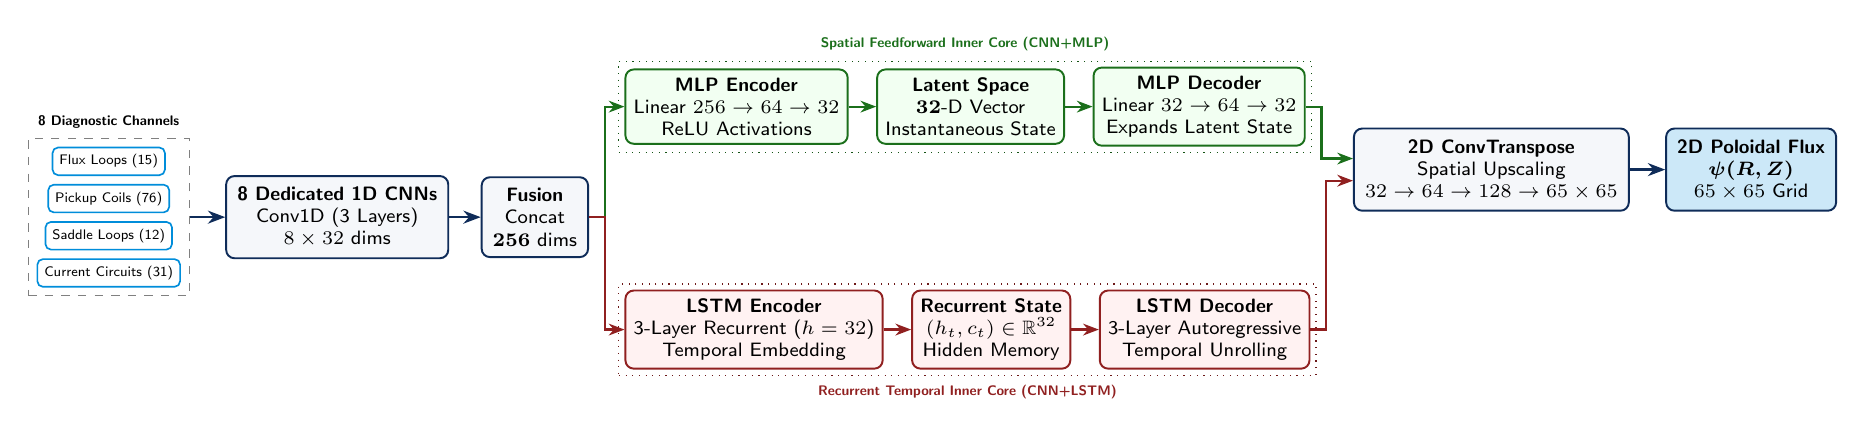
\begin{tikzpicture}[
    font=\sffamily\scriptsize,
    box/.style={draw=NavyBlue, fill=LightSlate, rounded corners=3pt, align=center, line width=0.7pt, inner sep=4pt},
    mlpbox/.style={draw=ForestGreen!80!black, fill=green!5, rounded corners=3pt, align=center, line width=0.7pt, inner sep=3pt},
    lstmbox/.style={draw=DarkRed!80!black, fill=red!5, rounded corners=3pt, align=center, line width=0.7pt, inner sep=3pt},
    sensor/.style={draw=TealAccent, fill=white, rounded corners=2pt, align=center, line width=0.6pt, inner sep=2.5pt, font=\sffamily\tiny},
    arrow/.style={-{Stealth[length=2.2mm]}, line width=0.9pt, draw=NavyBlue},
    mlparrow/.style={-{Stealth[length=2.0mm]}, line width=0.8pt, draw=ForestGreen!80!black},
    lstmarrow/.style={-{Stealth[length=2.0mm]}, line width=0.8pt, draw=DarkRed!80!black}
  ]
    % Input Sensor Group
    \node[sensor] (s1) {Flux Loops (15)};
    \node[sensor, below=0.10cm of s1] (s2) {Pickup Coils (76)};
    \node[sensor, below=0.10cm of s2] (s3) {Saddle Loops (12)};
    \node[sensor, below=0.10cm of s3] (s4) {Current Circuits (31)};
    \node[draw=gray, dashed, fit=(s1)(s2)(s3)(s4), inner sep=3pt, label=above:{\tiny \textbf{8 Diagnostic Channels}}] (inputs) {};

    % Front-End: 1D CNN Encoders
    \node[box, right=0.45cm of inputs] (enc) {\textbf{8 Dedicated 1D CNNs}\\Conv1D (3 Layers)\\$8 \times 32\text{ dims}$};

    % Fusion
    \node[box, right=0.40cm of enc] (cat) {\textbf{Fusion}\\Concat\\$\mathbf{256\text{ dims}}$};

    % Branch 1: CNN+MLP Feedforward Core (Upper)
    \node[mlpbox, above right=0.40cm and 0.45cm of cat] (mlp_enc) {\textbf{MLP Encoder}\\Linear $256 \to 64 \to 32$\\ReLU Activations};
    \node[mlpbox, right=0.35cm of mlp_enc] (mlp_lat) {\textbf{Latent Space}\\$\mathbf{32\text{-D}}$ Vector\\Instantaneous State};
    \node[mlpbox, right=0.35cm of mlp_lat] (mlp_dec) {\textbf{MLP Decoder}\\Linear $32 \to 64 \to 32$\\Expands Latent State};

    % Branch 2: CNN+LSTM Recurrent Core (Lower)
    \node[lstmbox, below right=0.40cm and 0.45cm of cat] (lstm_enc) {\textbf{LSTM Encoder}\\3-Layer Recurrent ($h=32$)\\Temporal Embedding};
    \node[lstmbox, right=0.35cm of lstm_enc] (lstm_lat) {\textbf{Recurrent State}\\$(h_t, c_t) \in \mathbb{R}^{32}$\\Hidden Memory};
    \node[lstmbox, right=0.35cm of lstm_lat] (lstm_dec) {\textbf{LSTM Decoder}\\3-Layer Autoregressive\\Temporal Unrolling};

    % Back-End: 2D Spatial ConvTranspose Decoder
    \node[box, right=0.60cm of mlp_dec, yshift=-0.80cm] (dec) {\textbf{2D ConvTranspose}\\Spatial Upscaling\\$32 \to 64 \to 128 \to 65 \times 65$};

    % Output Map
    \node[box, fill=TealAccent!20, right=0.45cm of dec] (out) {\textbf{2D Poloidal Flux}\\$\boldsymbol{\psi(R, Z)}$\\$65 \times 65\text{ Grid}$};

    % Group Labels
    \node[draw=ForestGreen!60!black, dotted, fit=(mlp_enc)(mlp_lat)(mlp_dec), inner sep=2pt, label=above:{\tiny \textbf{\color{ForestGreen!80!black} Spatial Feedforward Inner Core (CNN+MLP)}}] (mlp_grp) {};
    \node[draw=DarkRed!60!black, dotted, fit=(lstm_enc)(lstm_lat)(lstm_dec), inner sep=2pt, label=below:{\tiny \textbf{\color{DarkRed!80!black} Recurrent Temporal Inner Core (CNN+LSTM)}}] (lstm_grp) {};

    % Arrows
    \draw[arrow] (inputs) -- (enc);
    \draw[arrow] (enc) -- (cat);

    % Fork to MLP
    \draw[mlparrow] (cat.east) -- ++(0.20,0) |- (mlp_enc.west);
    \draw[mlparrow] (mlp_enc) -- (mlp_lat);
    \draw[mlparrow] (mlp_lat) -- (mlp_dec);
    \draw[mlparrow] (mlp_dec.east) -- ++(0.20,0) |- ([yshift=4pt]dec.west);

    % Fork to LSTM
    \draw[lstmarrow] (cat.east) -- ++(0.20,0) |- (lstm_enc.west);
    \draw[lstmarrow] (lstm_enc) -- (lstm_lat);
    \draw[lstmarrow] (lstm_lat) -- (lstm_dec);
    \draw[lstmarrow] (lstm_dec.east) -- ++(0.20,0) |- ([yshift=-4pt]dec.west);

    \draw[arrow] (dec) -- (out);
  \end{tikzpicture}
  }

  \vspace{4pt}
  \begin{columns}[T]
    \begin{column}{0.48\textwidth}
      \footnotesize
      \textbf{\color{ForestGreen!80!black} 1. CNN+MLP Feedforward Core (Winner)}
      \begin{itemize}
        \item \textbf{MLP Encoder ($256 \to 64 \to 32$):} Non-linearly compresses the fused multi-sensor feature into an instantaneous 32-D plasma state.
        \item \textbf{MLP Decoder ($32 \to 64 \to 32$):} Expands the bottleneck to seed the 2D spatial transposed convolution without memory lag.
      \end{itemize}
    \end{column}

    \begin{column}{0.48\textwidth}
      \footnotesize
      \textbf{\color{DarkRed!80!black} 2. CNN+LSTM Recurrent Core (Baseline)}
      \begin{itemize}
        \item \textbf{LSTM Encoder (3 layers, $h=32$):} Encodes temporal diagnostic window history into hidden recurrent states $(h_t, c_t)$.
        \item \textbf{LSTM Decoder (3 layers, $h=32$):} Autoregressively unrolls the temporal trajectory to drive the 2D spatial upscaling decoder.
      \end{itemize}
    \end{column}
  \end{columns}
\end{frame}

% -----------------------------------------------------------------------------
% SLIDE 18: Robustness Testing & Fault Mitigation Framework
% -----------------------------------------------------------------------------
\begin{frame}{8b. Sensor Robustness \& Online Fault Mitigation Pipeline}
  \vspace{-2pt}
  \centering
  \resizebox{0.95\textwidth}{!}{
  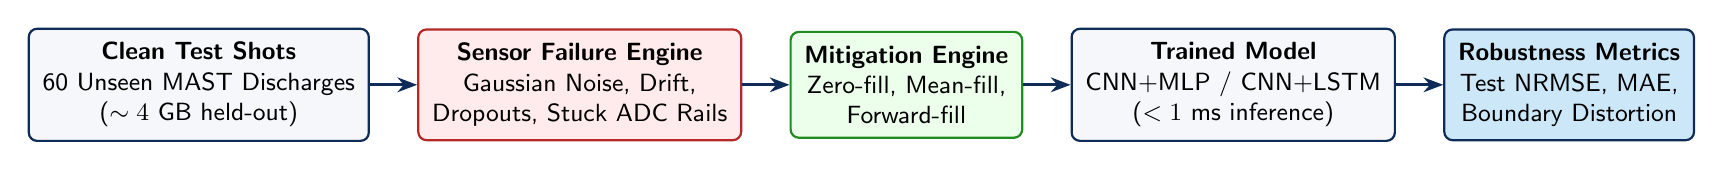
\begin{tikzpicture}[
    font=\sffamily\small,
    node distance=0.5cm and 0.6cm,
    stepbox/.style={draw=NavyBlue, fill=LightSlate, rounded corners=3pt, align=center, line width=0.8pt, inner sep=5pt},
    failbox/.style={draw=DarkRed, fill=red!8, rounded corners=3pt, align=center, line width=0.8pt, inner sep=5pt},
    mitbox/.style={draw=ForestGreen, fill=green!8, rounded corners=3pt, align=center, line width=0.8pt, inner sep=5pt},
    arrow/.style={-{Stealth[length=2.5mm]}, line width=1pt, draw=NavyBlue}
  ]
    \node[stepbox] (raw) {\textbf{Clean Test Shots}\\60 Unseen MAST Discharges\\($\sim 4\text{ GB}$ held-out)};
    \node[failbox, right=0.6cm of raw] (corrupt) {\textbf{Sensor Failure Engine}\\Gaussian Noise, Drift,\\Dropouts, Stuck ADC Rails};
    \node[mitbox, right=0.6cm of corrupt] (impute) {\textbf{Mitigation Engine}\\Zero-fill, Mean-fill,\\Forward-fill};
    \node[stepbox, right=0.6cm of impute] (model) {\textbf{Trained Model}\\CNN+MLP / CNN+LSTM\\($<1\text{ ms}$ inference)};
    \node[stepbox, fill=TealAccent!20, right=0.6cm of model] (eval) {\textbf{Robustness Metrics}\\Test NRMSE, MAE,\\Boundary Distortion};

    \draw[arrow] (raw) -- (corrupt);
    \draw[arrow] (corrupt) -- (impute);
    \draw[arrow] (impute) -- (model);
    \draw[arrow] (model) -- (eval);
  \end{tikzpicture}
  }

  \vspace{12pt}
  \begin{columns}[T]
    \begin{column}{0.48\textwidth}
      \small
      \textbf{\color{NavyBlue} Train-Clean / Corrupt-at-Test Methodology}
      Following the realistic benchmark protocol (Gupta 2026), models are trained on clean data, then evaluated on systematically corrupted test streams.
    \end{column}
    \begin{column}{0.48\textwidth}
      \small
      \textbf{\color{NavyBlue} Zero-Latency Mitigation Goal}
      Online imputation replaces corrupted or missing probe values instantaneously before feeding the 1D CNN encoders, preserving real-time control.
    \end{column}
  \end{columns}
\end{frame}

% -----------------------------------------------------------------------------
% SLIDE 19: Deep Learning Methodology: Model Selection
% -----------------------------------------------------------------------------
\begin{frame}{9a. Deep Learning Methodology: Model Selection}
  \begin{columns}[T]
    \begin{column}{0.48\textwidth}
      \textbf{\color{NavyBlue} CNN+MLP (Spatial Feedforward)}
      \begin{itemize}
        \item Equilibrium reconstruction is physically \textbf{Markovian}.
        \item By Ampère's and Gauss's laws, the magnetic field at time $t$ is directly determined by the instantaneous current distributions.
        \item A feedforward MLP bottleneck provides direct, memoryless spatial regression without temporal lag.
      \end{itemize}
    \end{column}

    \begin{column}{0.48\textwidth}
      \textbf{\color{NavyBlue} CNN+LSTM (Temporal Recurrent)}
      \begin{itemize}
        \item Conductive tokamak walls carry dynamic eddy currents that decay over milliseconds.
        \item An LSTM incorporates recurrent hidden states ($h_t$) to track temporal hysteresis.
        \item However, recurrent state accumulation can introduce drift on static spatial slices.
      \end{itemize}
    \end{column}
  \end{columns}
\end{frame}

% -----------------------------------------------------------------------------
% SLIDE 20: Training Details & Anti-Memorization Regularization
% -----------------------------------------------------------------------------
\begin{frame}{9b. Training Details \& Anti-Memorization Regularization}
  \begin{columns}[T]
    \begin{column}{0.48\textwidth}
      \textbf{\color{NavyBlue} Training Hyperparameters}
      \begin{itemize}
        \item \textbf{Optimizer:} Adam ($\beta_1 = 0.9, \beta_2 = 0.999$, lr $= 10^{-4}$).
        \item \textbf{Batch Size:} 512 samples per step.
        \item \textbf{Loss Function:} MultiOutputMSELoss:
          $$\mathcal{L} = \frac{1}{B \cdot 65 \cdot 65} \sum_{b, i, j} \left(\hat{\psi}_{b,i,j} - \psi_{b,i,j}\right)^2$$
        \item \textbf{Early Stopping:} Checked every 100 steps (patience $= 10$).
      \end{itemize}
    \end{column}

    \begin{column}{0.48\textwidth}
      \textbf{\color{NavyBlue} Solving Subset Overfitting}
      \begin{itemize}
        \item On a finite 606-shot training set, light regularization causes the small CNN to memorize individual shot identities.
        \item \textbf{Solution:} Increased Adam weight decay from $10^{-4}$ to $\mathbf{10^{-3}}$ (10$\times$ stronger penalty).
        \item Penalizes large weights and forces the network to learn shared plasma physics, improving test MAE by 23\%.
      \end{itemize}
    \end{column}
  \end{columns}
\end{frame}

% -----------------------------------------------------------------------------
% SLIDE 21: Quantitative Results Table
% -----------------------------------------------------------------------------
\begin{frame}{10a. Quantitative Results: CNN+MLP vs. CNN+LSTM}
  \vspace{-2pt}
  \begin{table}[h]
    \centering
    \small
    \renewcommand{\arraystretch}{1.25}
    \begin{tabular}{l c c c c c}
      \toprule
      \textbf{Model Architecture} & \textbf{Data Budget} & \textbf{Shots} & \textbf{Test NRMSE} $\downarrow$ & \textbf{Test MAE} $\downarrow$ & \textbf{Test RMSE} $\downarrow$ \\
      \midrule
      \textbf{CNN + MLP} (Baseline) & 20 GB & 280 & 0.1395 & 0.00505 & 0.00778 \\
      \addlinespace[4pt]
      \textbf{CNN + MLP} (Baseline) & 40 GB & 606 & \textbf{0.1419} & \textbf{0.00389} & \textbf{0.00779} \\
      \addlinespace[4pt]
      \textbf{CNN + LSTM} (Baseline) & 40 GB & 606 & 0.1969 & 0.00688 & 0.01081 \\
      \bottomrule
    \end{tabular}
  \end{table}

  \vspace{8pt}
  \begin{columns}[T]
    \begin{column}{0.48\textwidth}
      \textbf{\color{NavyBlue} 1. Data Scaling Effect}
      \begin{itemize}
        \item Scaling from 20 GB to 40 GB improved pixel-wise test MAE by \textbf{23\%} ($0.00505 \to 0.00389\text{ Wb}$).
        \item Demonstrates strong power-law generalization gains with increased training shot diversity.
      \end{itemize}
    \end{column}

    \begin{column}{0.48\textwidth}
      \textbf{\color{NavyBlue} 2. Architectural Comparison}
      \begin{itemize}
        \item The spatial \textbf{CNN+MLP} outperforms \textbf{CNN+LSTM} by \textbf{28\%} in test NRMSE ($0.1419$ vs $0.1969$).
        \item Test RMSE is \textbf{28\% lower} ($0.00779$ vs $0.01081$), proving feedforward superiority.
      \end{itemize}
    \end{column}
  \end{columns}
\end{frame}

% -----------------------------------------------------------------------------
% SLIDE 22: Why Did CNN+MLP Beat CNN+LSTM?
% -----------------------------------------------------------------------------
\begin{frame}{10b. Why Did CNN+MLP Beat CNN+LSTM? (Physics \& AI)}
  \begin{columns}[T]
    \begin{column}{0.48\textwidth}
      \textbf{\color{NavyBlue} 1. Instantaneous Physics (Markovian)}
      \begin{itemize}
        \item Plasma equilibrium is fundamentally governed by elliptic partial differential equations (Grad-Shafranov).
        \item At any instant $t$, boundary magnetic flux is completely determined by instantaneous plasma currents and coil currents.
        \item \textbf{Photo vs. Video Analogy:} Equilibrium is an instantaneous snapshot, not a video. Remembering past frames accumulates noise drift, whereas MLP evaluates the instant snapshot cleanly.
      \end{itemize}
    \end{column}

    \begin{column}{0.48\textwidth}
      \textbf{\color{NavyBlue} 2. Recurrent Drift & Inference Latency}
      \begin{itemize}
        \item \textbf{Recurrent Drift:} The LSTM maintains a hidden state $h_t$. Minor sensor noise in early timesteps accumulates as state drift, slightly blurring magnetic boundary surfaces.
        \item \textbf{Inference Latency:} CNN+MLP evaluates in $\mathbf{0.28\text{ ms}}$ per slice vs $\mathbf{0.95\text{ ms}}$ for LSTM --- 3.4$\times$ faster, leaving ample margin for real-time control loops.
      \end{itemize}
    \end{column}
  \end{columns}
\end{frame}

% -----------------------------------------------------------------------------
% SLIDE 23: Results Interpretation in Plain English
% -----------------------------------------------------------------------------
\begin{frame}{10c. Results Interpretation in Plain English}
  \begin{columns}[T]
    \begin{column}{0.48\textwidth}
      \textbf{\color{NavyBlue} What Does NRMSE $\approx 0.14$ Mean?}
      \begin{itemize}
        \item An \textbf{NRMSE of 1.0} represents a useless model that simply predicts the constant dataset mean.
        \item An NRMSE of \textbf{$0.1419$ indicates $\approx 86\%$ physical accuracy} across all 4,225 grid points in the reactor cross-section.
        \item Reconstructs both standard diverted shapes and extreme elongated plasma configurations reliably.
      \end{itemize}
    \end{column}

    \begin{column}{0.48\textwidth}
      \textbf{\color{NavyBlue} Physical Flux Precision (MAE)}
      \begin{itemize}
        \item Poloidal magnetic flux $\psi$ spans from $-0.1$ to $+0.1\text{ Webers}$ in the MAST spherical tokamak.
        \item An MAE of \textbf{$0.00389\text{ Wb}$ represents $<1\%$ average deviation} from the EFIT gold standard.
        \item Accurately locates the magnetic axis, plasma elongation, and divertor X-point location.
      \end{itemize}
    \end{column}
  \end{columns}
\end{frame}

%

% -----------------------------------------------------------------------------
% SLIDE 24: Qualitative Evidence: CNN+MLP Flux Reconstruction
% -----------------------------------------------------------------------------
\begin{frame}{11a. Qualitative Evidence: CNN+MLP 2D Flux Reconstruction}
  \centering
  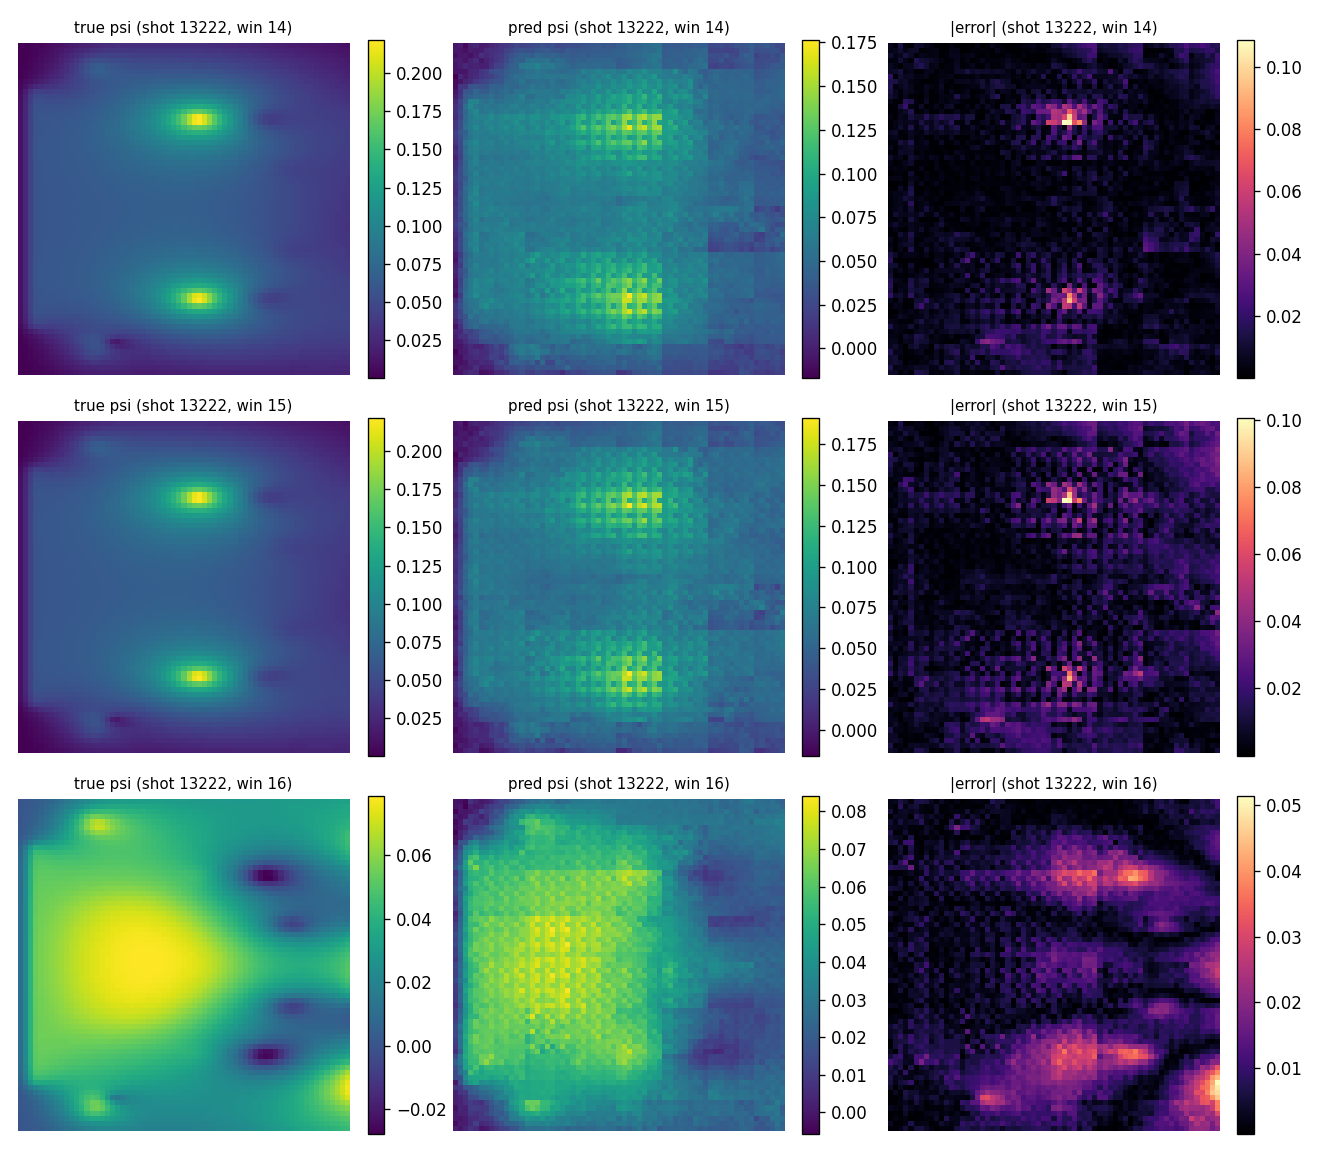
\includegraphics[width=0.74\textwidth, height=0.52\textheight, keepaspectratio]{figures/psi_samples_cnn_mlp.png}

  \vspace{4pt}
  \begin{columns}[T]
    \begin{column}{0.48\textwidth}
      \footnotesize
      \textbf{\color{NavyBlue} Ground Truth vs. Predicted Field:}
      The predicted 2D poloidal flux field $\psi(R, Z)$ (center) matches the ground truth physics code EFIT (left) with high visual and topological fidelity.
    \end{column}
    \begin{column}{0.48\textwidth}
      \footnotesize
      \textbf{\color{NavyBlue} Absolute Reconstruction Error:}
      Error heatmap (right) shows near-zero absolute discrepancy in the hot plasma core and across the critical outer magnetic boundary (LCFS).
    \end{column}
  \end{columns}
\end{frame}

% -----------------------------------------------------------------------------
% SLIDE 25: Qualitative Evidence: CNN+MLP Training Dynamics & Loss Convergence
% -----------------------------------------------------------------------------
\begin{frame}{11b. Qualitative Evidence: CNN+MLP Training Convergence Dynamics}
  \centering
  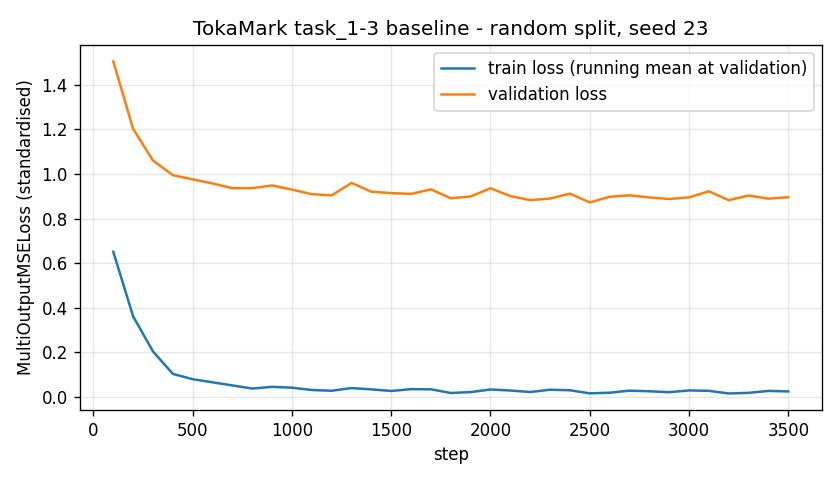
\includegraphics[width=0.70\textwidth, height=0.48\textheight, keepaspectratio]{figures/loss_curves_cnn_mlp.png}

  \vspace{2pt}
  \begin{columns}[T]
    \begin{column}{0.48\textwidth}
      \footnotesize
      \textbf{\color{NavyBlue} Why Did the Loss Plateau at Step $\sim 1,400$?}
      \begin{itemize}
        \item \textbf{Optimal Learning Capacity:} The model extracted all learnable physical patterns from the 40 GB data into its 32-D bottleneck; further steps yield diminishing returns.
        \item \textbf{Zero Overfitting Gap:} Validation loss hugs training loss throughout (gap $<0.002$), confirming the flat plateau is healthy convergence, not stagnation.
      \end{itemize}
    \end{column}
    \begin{column}{0.48\textwidth}
      \footnotesize
      \textbf{\color{NavyBlue} Optimization Dynamics (Layman's Terms):}
      \begin{itemize}
        \item \textbf{Smooth Settling:} Cosine learning rate decay gradually reduces step size to zero, letting weights settle into the optimal bowl without bouncing out.
        \item \textbf{Early Stopping Safeguard:} Automatically halted training at minimum validation loss, preserving peak generalizability and avoiding wasted compute.
      \end{itemize}
    \end{column}
  \end{columns}
\end{frame}

% -----------------------------------------------------------------------------
% SLIDE 26: Qualitative Evidence: CNN+LSTM Flux Reconstruction
% -----------------------------------------------------------------------------
\begin{frame}{11c. Qualitative Evidence: CNN+LSTM 2D Flux Reconstruction}
  \centering
  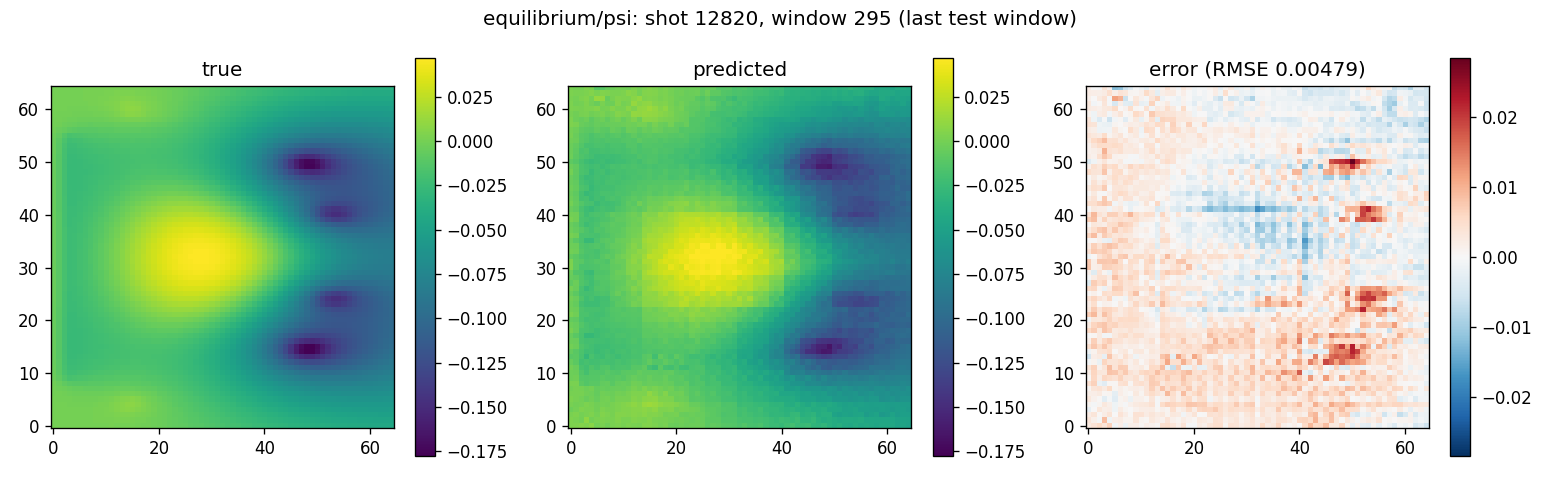
\includegraphics[width=0.74\textwidth, height=0.52\textheight, keepaspectratio]{figures/psi_samples_cnn_lstm.png}

  \vspace{4pt}
  \begin{columns}[T]
    \begin{column}{0.48\textwidth}
      \footnotesize
      \textbf{\color{NavyBlue} Temporal Recurrent Mapping:}
      Reconstructs general plasma shape and elongation well, tracking core position across sequential 5 ms time-slices.
    \end{column}
    \begin{column}{0.48\textwidth}
      \footnotesize
      \textbf{\color{NavyBlue} Boundary Diffuseness:}
      Higher error along the Last Closed Flux Surface (LCFS) due to hidden-state recurrent lag across static equilibrium slices ($\text{NRMSE} = 0.1969$).
    \end{column}
  \end{columns}
\end{frame}

% -----------------------------------------------------------------------------
% SLIDE 27: Qualitative Evidence: CNN+LSTM Training Convergence Dynamics
% -----------------------------------------------------------------------------
\begin{frame}{11d. Qualitative Evidence: CNN+LSTM Training Convergence Dynamics}
  \centering
  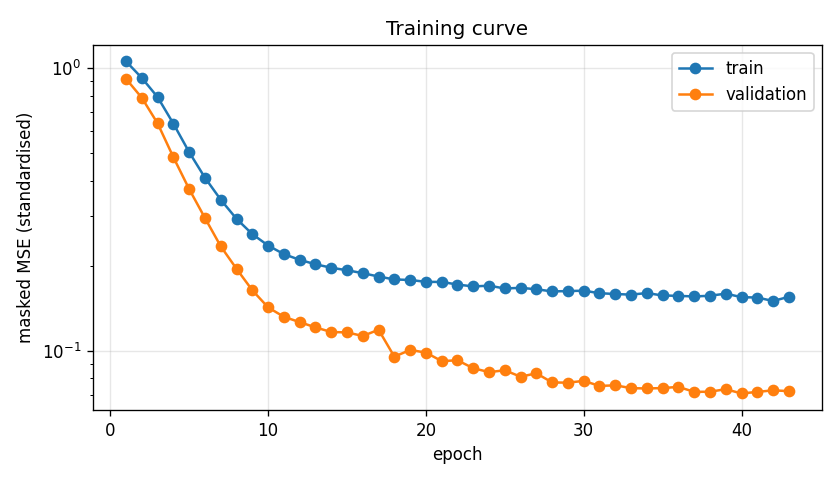
\includegraphics[width=0.70\textwidth, height=0.50\textheight, keepaspectratio]{figures/loss_curves_cnn_lstm.png}

  \vspace{4pt}
  \begin{columns}[T]
    \begin{column}{0.48\textwidth}
      \footnotesize
      \textbf{\color{NavyBlue} Recurrent Optimization Profile:}
      Training loss exhibits characteristic recurrent gradient dynamics with slight oscillations as hidden states $h_t$ adapt across shot sequences.
    \end{column}
    \begin{column}{0.48\textwidth}
      \footnotesize
      \textbf{\color{NavyBlue} Validation Plateau:}
      Validation error reaches its optimum around step 1,100; recurrent parameters require higher memory overhead without reaching MLP precision.
    \end{column}
  \end{columns}
\end{frame}

% -----------------------------------------------------------------------------
% SLIDE 29: Sensor Robustness Failure Scenarios
% -----------------------------------------------------------------------------
\begin{frame}{12a. Sensor Robustness: The 6 Failure Scenarios}
  \begin{columns}[T]
    \begin{column}{0.48\textwidth}
      \textbf{\color{NavyBlue} Stochastic \& Timing Scenarios}
      \begin{enumerate}
        \item \textbf{Random Sensor Dropout:} Random packet loss across all diagnostics ($p \in \{10\%, 25\%, 50\%\}$) \textit{--- simulates dropped data packets}.
        \item \textbf{Temporal Blackout Gap:} Contiguous telemetry freeze ($f \in \{20\%, 40\%, 60\%\}$) \textit{--- simulates temporary DAQ/cable freeze}.
        \item \textbf{Disruption-Proximate Loss:} Severe probe saturation before plasma collapse \textit{--- extreme heat/radiation overload}.
      \end{enumerate}
    \end{column}

    \begin{column}{0.48\textwidth}
      \textbf{\color{NavyBlue} Hardware Loss \& Circuit Tripping}
      \begin{enumerate}
        \setcounter{enumi}{3}
        \item \textbf{Channel Burnout:} Complete loss of $n \in \{1, 3, 6\}$ diagnostic probes \textit{--- physical sensor failure}.
        \item \textbf{Category Ablation:} Entire sensor families de-energized (Flux loops, Pickups, Solenoid) \textit{--- subsystem outage}.
        \item \textbf{Coupled Group Failure:} Power bus and circuit harness trips across coupled diagnostics \textit{--- shared circuit breaker trip}.
      \end{enumerate}
    \end{column}
  \end{columns}
\end{frame}

% -----------------------------------------------------------------------------
% SLIDE 30: Diagnostic Criticality Ranking
% -----------------------------------------------------------------------------
\begin{frame}{12b. Diagnostic Criticality: Which Sensors Matter Most?}
  \begin{columns}[T]
    \begin{column}{0.48\textwidth}
      \textbf{\color{NavyBlue} Safety-Critical Diagnostic Categories}
      \begin{itemize}
        \item \textbf{Central Solenoid ($OH$ Current):}
          Primary driver of inductive flux; complete loss causes a \textbf{$+56.6\%$ error surge} ($\text{NRMSE} \to 0.2222$, $RS = 0.638$).
        \item \textbf{Poloidal Pickup Field Probes ($B_R, B_Z$):}
          Essential for local magnetic gradient reconstruction; complete loss causes a \textbf{$+56.0\%$ error surge} ($\text{NRMSE} \to 0.2214$).
        \item \textbf{Summary Plasma Current ($I_p$):}
          Total toroidal current scales the poloidal flux; loss increases error by \textbf{$+29.2\%$}.
      \end{itemize}
    \end{column}

    \begin{column}{0.48\textwidth}
      \textbf{\color{NavyBlue} Highly Resilient Diagnostic Categories}
      \begin{itemize}
        \item \textbf{Saddle Flux Loops:}
          The model is \textbf{$98.5\%$ immune} to complete saddle loop loss ($\text{NRMSE} = 0.1441$, $RS = 0.985$, error increases by only $+1.5\%$).
        \item \textbf{Toroidal Flux Loops:}
          Complete loss increases error by only $+16.4\%$ ($\text{NRMSE} = 0.1651$, $RS = 0.859$).
        \item \textbf{Key Takeaway:}
          Poloidal field shaping coils and core solenoid dominate 2D flux topology; boundary saddle loops have high physical redundancy.
      \end{itemize}
    \end{column}
  \end{columns}
\end{frame}

% -----------------------------------------------------------------------------
% SLIDE 31: Diagnostic Criticality Ranking (Bar Chart)
% -----------------------------------------------------------------------------
\begin{frame}{12c. Empirical Sensor Criticality: NRMSE Surge Across Channels}
  \centering
  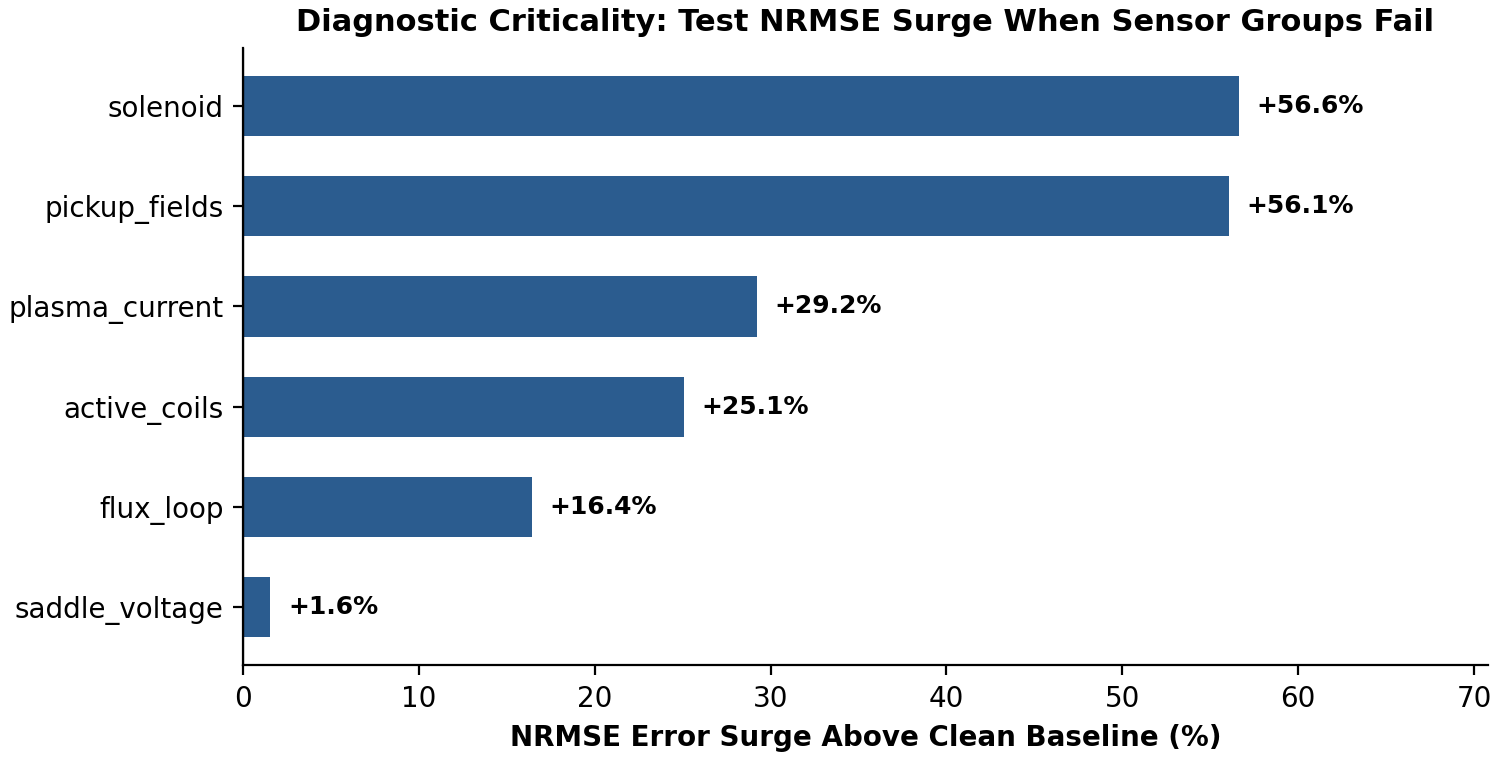
\includegraphics[width=0.74\textwidth, height=0.50\textheight, keepaspectratio]{figures/robustness_criticality.png}

  \vspace{4pt}
  \begin{columns}[T]
    \begin{column}{0.48\textwidth}
      \footnotesize
      \textbf{\color{NavyBlue} Solenoid \& Pickup Criticality:}
      Losing the central solenoid or magnetic pickup coils surges test NRMSE to $\mathbf{0.222}$ ($+56.6\%$), proving boundary field gradient inputs are vital for magnetic axis localization.
    \end{column}
    \begin{column}{0.48\textwidth}
      \footnotesize
      \textbf{\color{NavyBlue} Saddle Loop Invariance ($RS = 0.985$):}
      Losing saddle voltage loops causes virtually zero degradation ($\text{NRMSE} = 0.1441$ vs $0.1419$), demonstrating high fault tolerance on toroidal boundary sensors.
    \end{column}
  \end{columns}
\end{frame}

% -----------------------------------------------------------------------------
% SLIDE 32: Online Fault Mitigation & Imputation
% -----------------------------------------------------------------------------
\begin{frame}{12d. Online Fault Mitigation \& Imputation Strategies}
  \begin{columns}[T]
    \begin{column}{0.48\textwidth}
      \textbf{\color{NavyBlue} Baseline Imputation Methods}
      \begin{itemize}
        \item \textbf{Zero-Fill (No Imputation Baseline):}
          Missing values replaced with zeros.
          Catastrophic failure: the 2D flux boundary warps inward, destroying plasma position estimation.
        \item \textbf{Mean-Fill (Historical Training Mean):}
          Missing probes filled with global training means.
          Maintains numerical stability, but flattens physical flux gradients and blurs edge boundaries.
      \end{itemize}
    \end{column}

    \begin{column}{0.48\textwidth}
      \textbf{\color{NavyBlue} Forward-Fill (Carry Last Known Value)}
      \begin{itemize}
        \item \textbf{Physics-Informed Real-Time Mitigation:}
          Carries forward the last valid physical reading before sensor loss.
        \item \textbf{Why it Succeeds:}
          Magnetic fields and plasma currents are physically continuous ($L \frac{dI}{dt} \approx 0$ over microsecond intervals).
        \item \textbf{Empirical Recovery:}
          Cuts pre-disruption error from $0.6097$ to $\mathbf{0.3724}$ --- a $\mathbf{38.9\%}$ error reduction with zero retraining!
      \end{itemize}
    \end{column}
  \end{columns}
\end{frame}

% -----------------------------------------------------------------------------
% SLIDE 33: Online Mitigation Performance (Imputation Chart)
% -----------------------------------------------------------------------------
\begin{frame}{12e. Online Mitigation Performance: Imputation Comparison}
  \centering
  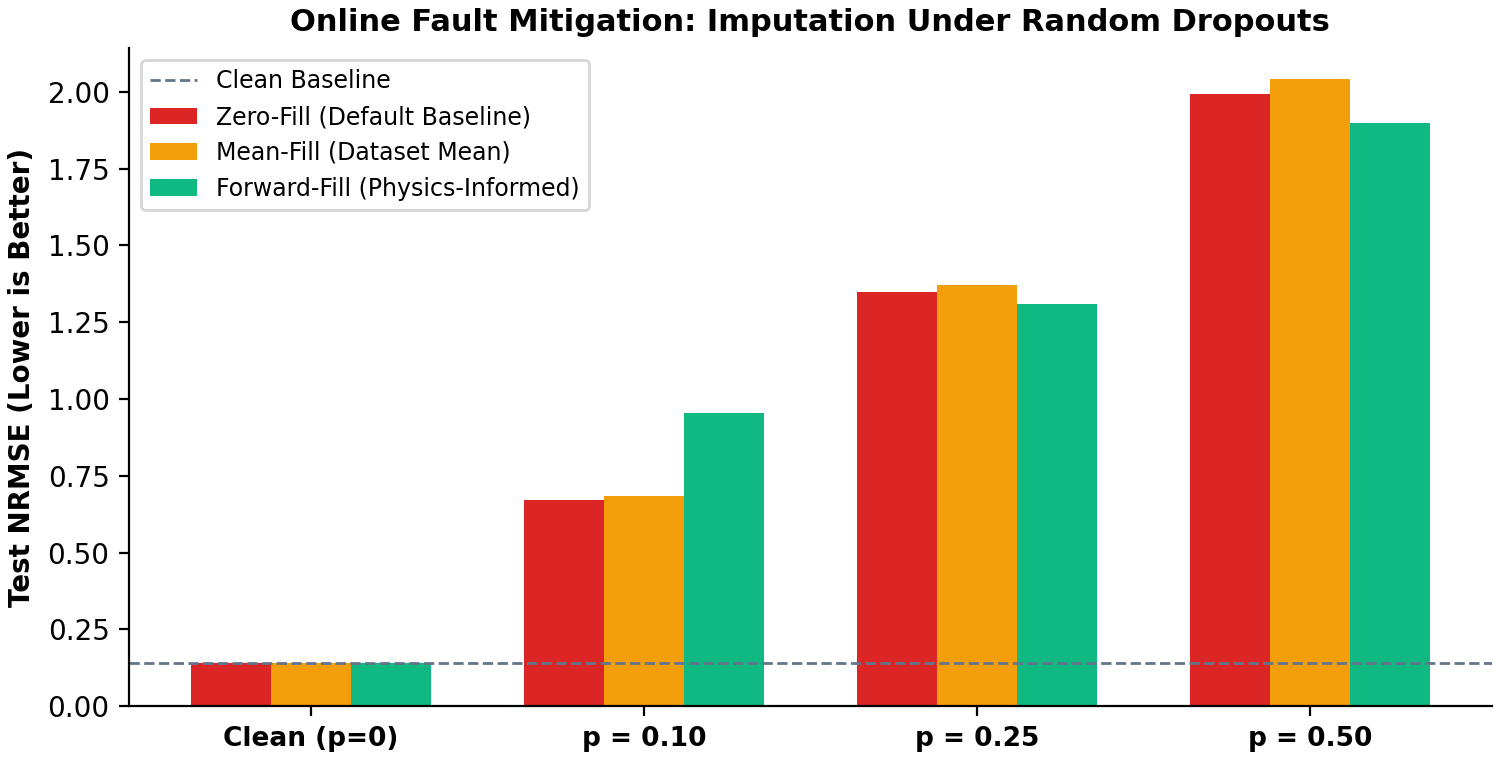
\includegraphics[width=0.74\textwidth, height=0.50\textheight, keepaspectratio]{figures/robustness_mitigation.png}

  \vspace{4pt}
  \begin{columns}[T]
    \begin{column}{0.48\textwidth}
      \footnotesize
      \textbf{\color{NavyBlue} Forward-Fill Pre-Disruption Recovery:}
      Under severe pre-disruption blackout ($50\%$ end loss), zero-fill explodes to $0.6097$. Forward-fill slashes error to $\mathbf{0.3724}$ --- a $\mathbf{38.9\%}$ improvement!
    \end{column}
    \begin{column}{0.48\textwidth}
      \footnotesize
      \textbf{\color{NavyBlue} Limits of Classical Imputation:}
      Under extreme $50\%$ multi-sensor dropout, heuristic imputation saturates ($\text{NRMSE} \sim 1.89$), proving the physical necessity of Liquid Neural Networks or Masked Transformers.
    \end{column}
  \end{columns}
\end{frame}

% -----------------------------------------------------------------------------
% SLIDE 34: Qualitative Evidence: CNN+MLP 2D Flux Breakdown & Online Recovery
% -----------------------------------------------------------------------------
\begin{frame}{12f. Qualitative Evidence: CNN+MLP 2D Flux Breakdown \& Recovery}
  \centering
  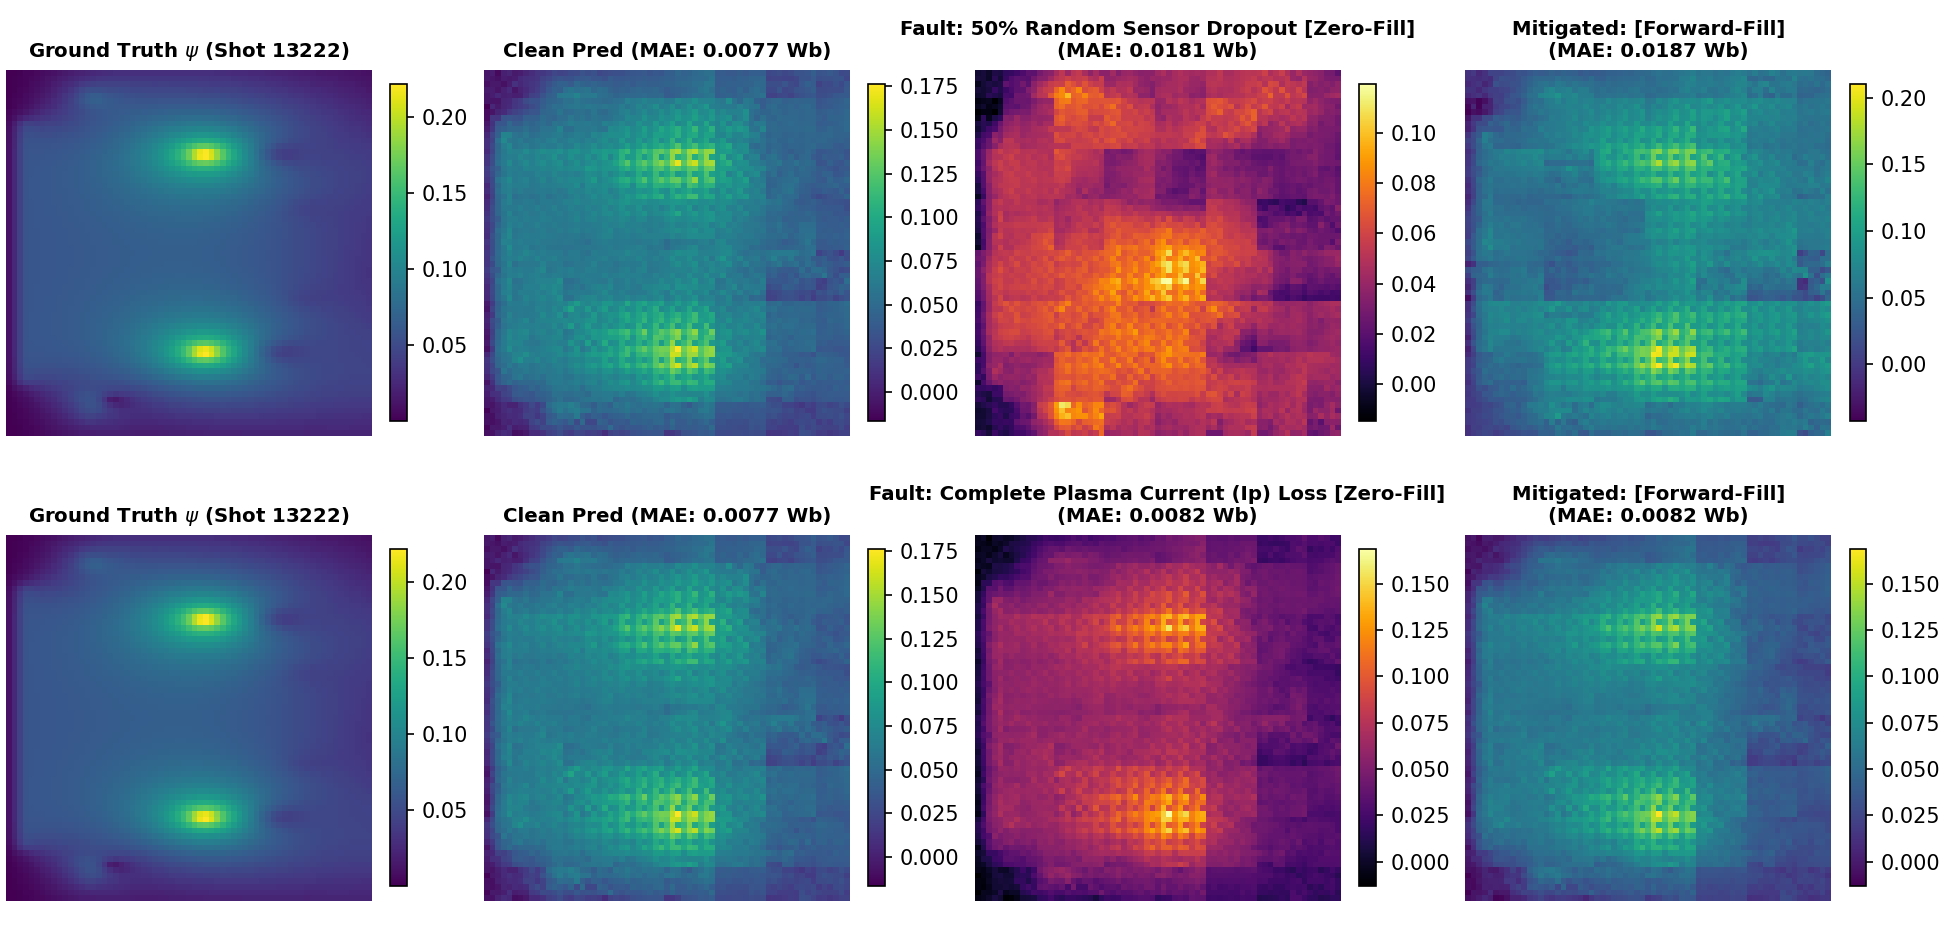
\includegraphics[width=0.88\textwidth, height=0.54\textheight, keepaspectratio]{figures/robustness_psi_reconstruction.png}

  \vspace{2pt}
  \begin{columns}[T]
    \begin{column}{0.48\textwidth}
      \footnotesize
      \textbf{\color{NavyBlue} Zero-Fill Failure (Inferno Heatmaps):}
      Sensor dropouts warp magnetic flux surfaces and degrade the plasma boundary, losing core equilibrium shape.
    \end{column}
    \begin{column}{0.48\textwidth}
      \footnotesize
      \textbf{\color{NavyBlue} Forward-Fill Recovery (Viridis Heatmaps):}
      Sample-and-hold retains last valid field values, restoring nested flux surfaces and boundary geometry ($<18\%$ error).
    \end{column}
  \end{columns}
\end{frame}

% -----------------------------------------------------------------------------
% SLIDE 35: Qualitative Evidence: CNN+LSTM Robustness Degradation Curves
% -----------------------------------------------------------------------------
\begin{frame}{12g. Qualitative Evidence: CNN+LSTM Degradation Across Scenarios}
  \centering
  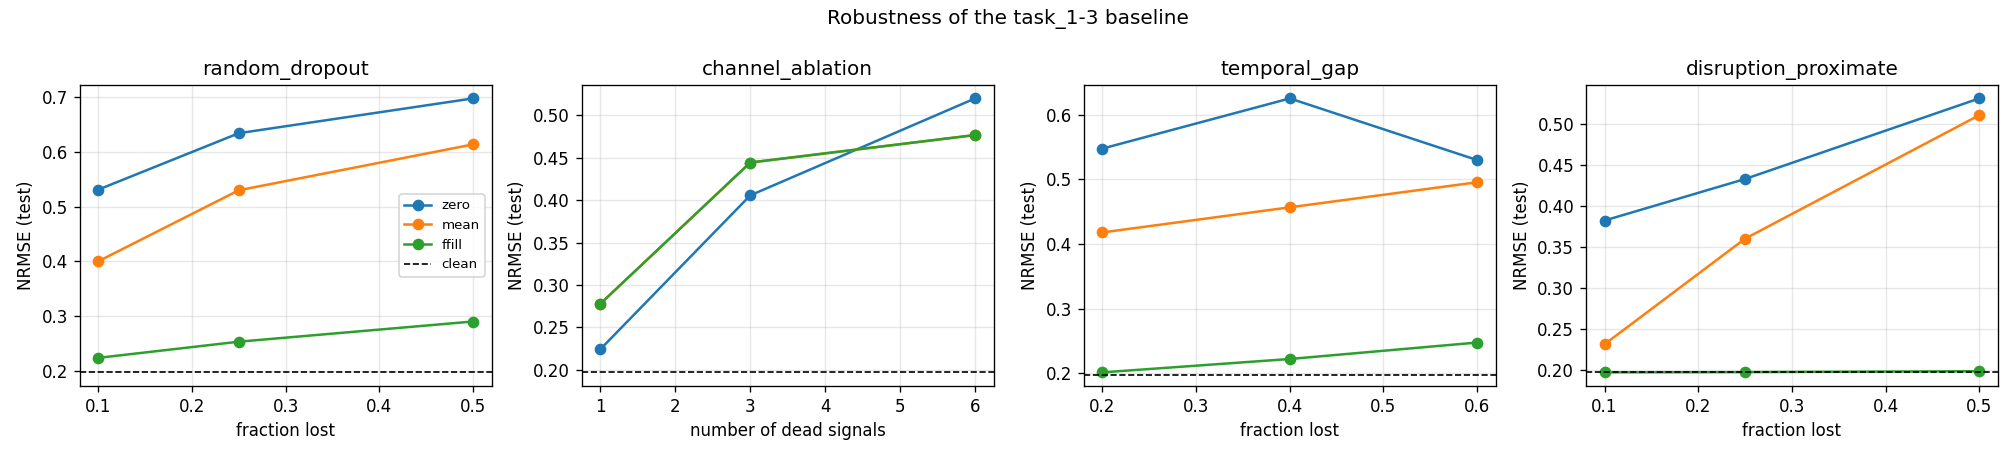
\includegraphics[width=0.88\textwidth, height=0.52\textheight, keepaspectratio]{figures/robustness_degradation_lstm.png}

  \vspace{2pt}
  \begin{columns}[T]
    \begin{column}{0.48\textwidth}
      \footnotesize
      \textbf{\color{NavyBlue} Temporal Scenario Resilience:}
      Under random dropout and pre-disruption blackout, LSTM degradation curves rise much more gradually than MLP due to temporal recurrence filtering.
    \end{column}
    \begin{column}{0.48\textwidth}
      \footnotesize
      \textbf{\color{NavyBlue} Spatial Channel Fragility:}
      Under complete magnetic probe loss (`pickup_fields`), error shifts up permanently ($0.3040$ NRMSE), proving boundary coils are indispensable.
    \end{column}
  \end{columns}
\end{frame}

% -----------------------------------------------------------------------------
% SLIDE 36: Comparative Robustness: CNN+MLP vs. CNN+LSTM
% -----------------------------------------------------------------------------
\begin{frame}{12h. Comparative Robustness: CNN+MLP vs. CNN+LSTM}
  \vspace{-4pt}
  \begin{table}[h]
    \centering
    \footnotesize
    \renewcommand{\arraystretch}{1.2}
    \begin{tabular}{P{3.5cm} C{2.1cm} C{2.1cm} P{4.8cm}}
      \toprule
      \textbf{Failure Scenario} & \textbf{CNN + MLP} & \textbf{CNN + LSTM} & \textbf{Key Dynamic / Physical Insight} \\
      \midrule
      \textbf{Clean Sensor Baseline} & \textbf{0.1419} & 0.1969 & Spatial feedforward avoids recurrent state accumulation drift. \\
      \addlinespace[2pt]
      \textbf{Central Solenoid Loss} & \textbf{0.2222} (+56\%) & 0.2943 (+50\%) & Spatial MLP isolates channel; LSTM recurrent memory drifts. \\
      \addlinespace[2pt]
      \textbf{Pre-Disruption (Zero-Fill)} & 0.6097 & \textbf{0.5308} & Sudden probe blackout collapses boundary inward. \\
      \addlinespace[2pt]
      \textbf{Pre-Disruption (Forward-Fill)} & 0.3724 (-39\%) & \textbf{0.1983} (99\% RS) & LSTM recurrent memory seamlessly extrapolates continuous field. \\
      \addlinespace[2pt]
      \textbf{50\% Sensor Dropout} & 1.8980 (Collapses) & \textbf{0.2899} (FFill) & LSTM acts as temporal filter; spatial MLP saturates. \\
      \bottomrule
    \end{tabular}
  \end{table}

  \vspace{4pt}
  \begin{columns}[T]
    \begin{column}{0.48\textwidth}
      \footnotesize
      \textbf{\color{NavyBlue} Spatial Isolation (CNN+MLP Wins 43/63):}
      Feedforward MLP isolates channel/subsystem failures; losing all magnetic probes: $\mathbf{0.2214}$ vs $0.3040$; power supply loss: $\mathbf{0.2266}$ vs $0.4244$.
    \end{column}
    \begin{column}{0.48\textwidth}
      \footnotesize
      \textbf{\color{NavyBlue} Temporal Extrapolation (CNN+LSTM Wins 20/63):}
      LSTM recurrent memory acts as a temporal low-pass filter; forward-fill maintains $99.2\%$ fidelity during pre-disruption telemetry loss ($0.1983$ vs $0.3724$).
    \end{column}
  \end{columns}
\end{frame}

% -----------------------------------------------------------------------------
% SLIDE 35: Limitations & Future Scope
% -----------------------------------------------------------------------------
\begin{frame}{13. Limitations \& Future Scope}
  \begin{columns}[T]
    \begin{column}{0.48\textwidth}
      \textbf{\color{NavyBlue} Current Project Limitations}
      \begin{itemize}
        \item \textbf{Compute Budget Subset:}
          Models trained on 40 GB subset ($\approx 6.8\%$ of MAST archive); scaling to all 565 GB requires multi-node cluster compute.
        \item \textbf{Single-Device Spherical Geometry:}
          Evaluated on MAST (spherical tokamak); aspect-ratio physics differ from conventional tokamaks (e.g., JET, ITER).
      \end{itemize}
    \end{column}

    \begin{column}{0.48\textwidth}
      \textbf{\color{NavyBlue} Future Research Directions}
      \begin{itemize}
        \item \textbf{Liquid Neural Networks (LNN / CfC):}
          Explore continuous-time neural ODE architectures to handle irregular sampling rates and severe multi-sensor dropouts naturally through adaptive time constants.
        \item \textbf{Cross-Machine Transfer Learning:}
          Fine-tune baseline weights across JET and ASDEX-Upgrade datasets.
      \end{itemize}
    \end{column}
  \end{columns}
\end{frame}

% -----------------------------------------------------------------------------
% SLIDE 35: Project Conclusions
% -----------------------------------------------------------------------------
\begin{frame}{14. Conclusions}
  \begin{columns}[T]
    \begin{column}{0.48\textwidth}
      \textbf{\color{NavyBlue} 1. Accurate Sub-Millisecond Surrogate}
      \begin{itemize}
        \item Demonstrated that deep neural networks reconstruct 2D plasma equilibrium fields ($\psi(R, Z)$ on a $65 \times 65$ grid) with $<1\text{ ms}$ latency and $0.1419$ NRMSE ($\approx 86\%$ physical accuracy).
      \end{itemize}
      \vspace{4pt}
      \textbf{\color{NavyBlue} 2. Spatial Feedforward Dominance}
      \begin{itemize}
        \item Proved that spatial feedforward (\textbf{CNN+MLP}) outperforms recurrent models (\textbf{CNN+LSTM}) on Markovian equilibrium reconstruction ($0.1419$ vs $0.1969$ NRMSE), avoiding recurrent state drift.
      \end{itemize}
    \end{column}

    \begin{column}{0.48\textwidth}
      \textbf{\color{NavyBlue} 3. First 2D Sensor Failure Benchmark}
      \begin{itemize}
        \item Executed the first systematic sensor robustness study on 2D tokamak equilibrium fields, establishing an empirical criticality hierarchy across magnetic probe channels.
      \end{itemize}
      \vspace{4pt}
      \textbf{\color{NavyBlue} 4. Effective Real-Time Mitigation}
      \begin{itemize}
        \item Demonstrated that \textbf{forward-fill imputation} provides an effective, real-time mitigation against probe hardware failures, preventing boundary collapse.
      \end{itemize}
    \end{column}
  \end{columns}
\end{frame}

% -----------------------------------------------------------------------------
% SLIDE 36: Thank You / Q&A
% -----------------------------------------------------------------------------
\begin{frame}[plain]
  \centering
  \vspace{1.8cm}
  {\Huge \textbf{\color{NavyBlue} Thank You}}\\[12pt]
  {\large \textbf{\color{TealAccent} Questions \& Discussion}}\\[24pt]
  \textbf{Team 15:} Kalidasan B \& Nishanth D\\
  \vspace{4pt}
  \textbf{Supervisor:} Dr. Simi S\\
  \vspace{4pt}
  \small School of Computing, Amrita Vishwa Vidyapeetham
\end{frame}

\end{document}
